\documentclass[11pt,a4paper]{article}

% ---------------------------------------------------------------------------
% Packages
% ---------------------------------------------------------------------------
\usepackage[a4paper,margin=2.3cm,top=2.6cm,bottom=2.8cm]{geometry}
\usepackage{lmodern}
\usepackage{microtype}
\usepackage[T1]{fontenc}
\usepackage{xcolor}
\usepackage{booktabs}
\usepackage{array}
\usepackage{longtable}
\usepackage{enumitem}
\usepackage{titlesec}
\usepackage{titletoc}
\usepackage{fancyhdr}
\usepackage{tcolorbox}
\tcbuselibrary{skins,breakable}
\usepackage{tikz}
\usetikzlibrary{arrows.meta,positioning,calc,automata,shapes.multipart}
\usepackage[colorlinks=true,linkcolor=accentlink,urlcolor=accentlink,citecolor=accentlink,linktoc=all]{hyperref}
\usepackage{parskip}
\usepackage{caption}
\usepackage{amsmath}

% ---------------------------------------------------------------------------
% Palette
% ---------------------------------------------------------------------------
\definecolor{accent}{HTML}{1F4E79}
\definecolor{accentlink}{HTML}{1F4E79}
\definecolor{accentlight}{HTML}{DCE8F2}
\definecolor{accentmid}{HTML}{6699CC}
\definecolor{paper}{HTML}{FFFFFF}
\definecolor{inkgray}{HTML}{333333}
\definecolor{warnbg}{HTML}{FFF6E5}
\definecolor{warnframe}{HTML}{C98A1B}
\definecolor{sysbg}{HTML}{EFF6EC}
\definecolor{sysframe}{HTML}{4B8B3B}

\color{inkgray}

% ---------------------------------------------------------------------------
% Section styling
% ---------------------------------------------------------------------------
\titleformat{\section}
  {\normalfont\Large\bfseries\color{accent}}
  {\thesection}{0.6em}{}
  [\vspace{-0.3em}{\color{accentmid}\titlerule[1pt]}]
\titleformat{\subsection}
  {\normalfont\large\bfseries\color{accent}}
  {\thesubsection}{0.6em}{}
\titleformat{\subsubsection}
  {\normalfont\normalsize\bfseries\color{accent}}
  {\thesubsubsection}{0.6em}{}

\titlespacing*{\section}{0pt}{1.6em}{0.9em}
\titlespacing*{\subsection}{0pt}{1.2em}{0.6em}

% ---------------------------------------------------------------------------
% Header / footer
% ---------------------------------------------------------------------------
\pagestyle{fancy}
\fancyhf{}
\renewcommand{\headrulewidth}{0.4pt}
\renewcommand{\footrulewidth}{0.4pt}
\fancyhead[L]{\small\color{accent}\textbf{RX --- Receiver Module}}
\fancyhead[R]{\small\color{inkgray}RTL Specification}
\fancyfoot[L]{\small\color{inkgray}rx-uvm-env}
\fancyfoot[C]{\small\color{inkgray}\thepage}
\fancyfoot[R]{\small\color{inkgray}Confidential}

\fancypagestyle{plain}{%
  \fancyhf{}
  \renewcommand{\headrulewidth}{0pt}
  \fancyfoot[C]{\small\color{inkgray}\thepage}
}

% ---------------------------------------------------------------------------
% Helper boxes
% ---------------------------------------------------------------------------
\newtcolorbox{noteBox}[1][]{
  enhanced, breakable, colback=accentlight, colframe=accentmid,
  boxrule=0.5pt, left=8pt, right=8pt, top=6pt, bottom=6pt,
  arc=2pt, title={#1}, fonttitle=\bfseries\color{accent},
  coltitle=accent, colbacktitle=accentlight,
  attach boxed title to top left={yshift=-2mm, xshift=6mm},
  boxed title style={colback=accentlight, colframe=accentlight},
}

\newtcolorbox{ruleBox}[1][]{
  enhanced, breakable, colback=warnbg, colframe=warnframe,
  boxrule=0.6pt, left=8pt, right=8pt, top=6pt, bottom=6pt, arc=2pt,
  title={#1}, fonttitle=\bfseries, coltitle=white,
}

\newtcolorbox{sysBox}[1][]{
  enhanced, breakable, colback=sysbg, colframe=sysframe,
  boxrule=0.6pt, left=8pt, right=8pt, top=5pt, bottom=5pt, arc=2pt,
  title={#1}, fonttitle=\bfseries, coltitle=white,
  before skip=8pt, after skip=8pt,
}

\newcolumntype{L}[1]{>{\raggedright\arraybackslash}p{#1}}
\newcolumntype{C}[1]{>{\centering\arraybackslash}p{#1}}

% ---------------------------------------------------------------------------
% Shared RX block diagram (used on the cover page and in Section 2.1)
% Arrowheads always point in the direction of signal flow: into the box
% for inputs (left side), out of the box for outputs (right side).
% ---------------------------------------------------------------------------
\newcommand{\RXDiagram}{
  \node[draw=accent, very thick, fill=accentlight, rounded corners=6pt,
        minimum width=4.6cm, minimum height=4.6cm, align=center]
        (rx) {\huge\bfseries\color{accent} RX};

  \coordinate (in1) at ([yshift=1.5cm]rx.west);
  \coordinate (in2) at ([yshift=0.5cm]rx.west);
  \coordinate (in3) at ([yshift=-0.7cm]rx.west);

  \draw[-{Latex[length=3mm]}, line width=1.4pt] ($(in1)+(-2.8,0)$) -- (in1);
  \node[left, align=right] at ($(in1)+(-2.8,0)$)
        {\texttt{input\_data}\\[-2pt]\scriptsize [3:0]};
  \draw[-{Latex[length=3mm]}] ($(in2)+(-2.8,0)$) -- (in2);
  \node[left, align=right] at ($(in2)+(-2.8,0)$)
        {\texttt{input\_valid}};
  \draw[-{Latex[length=3mm]}, line width=1.4pt] ($(in3)+(-2.8,0)$) -- (in3);
  \node[left, align=right] at ($(in3)+(-2.8,0)$)
        {\texttt{lock\_valid\_}\\[-2pt]\texttt{threshold}\\[-2pt]\scriptsize [15:0]};

  \draw[-{Latex[length=3mm]}, line width=1.4pt] (rx.east) ++(0,1.9) -- ++(2.8,0)
        node[right, align=left] {\texttt{output\_data}\\[-2pt]\scriptsize [31:0]};
  \draw[-{Latex[length=3mm]}] (rx.east) ++(0,1.15) -- ++(2.8,0)
        node[right, align=left] {\texttt{output\_valid}};
  \draw[-{Latex[length=3mm]}, line width=1.4pt] (rx.east) ++(0,0.4) -- ++(2.8,0)
        node[right, align=left] {\texttt{control\_out}\\[-2pt]\scriptsize [15:0]};
  \draw[-{Latex[length=3mm]}] (rx.east) ++(0,-0.35) -- ++(2.8,0)
        node[right, align=left] {\texttt{control\_valid}};
  \draw[-{Latex[length=3mm]}] (rx.east) ++(0,-1.1) -- ++(2.8,0)
        node[right, align=left] {\texttt{parity\_valid}};
  \draw[-{Latex[length=3mm]}] (rx.east) ++(0,-1.85) -- ++(2.8,0)
        node[right, align=left] {\texttt{parity\_not\_valid}};
}

% ---------------------------------------------------------------------------
% PDF metadata
% ---------------------------------------------------------------------------
\hypersetup{
  pdftitle={RX Receiver Module -- RTL Specification},
  pdfauthor={rx-uvm-env},
  pdfsubject={RX Block RTL Functional Specification},
}

\begin{document}

% ===========================================================================
% Cover page
% ===========================================================================
\begin{titlepage}
\newgeometry{top=0cm,bottom=2.5cm,left=2.5cm,right=2.5cm}
\begin{tikzpicture}[remember picture, overlay]
  \fill[accent] (current page.north west) rectangle
    ([yshift=-3.6cm]current page.north east);
  \fill[accentmid] ([yshift=-3.6cm]current page.north west) rectangle
    ([yshift=-3.75cm]current page.north east);
\end{tikzpicture}

\vspace{1.35cm}
{\color{white}\Huge\bfseries \hspace{0.2cm} RX --- Receiver Module}\\[0.3cm]
{\color{white}\Large \hspace{0.2cm} RTL Functional Specification}

\vspace{1.6cm}

\begin{center}
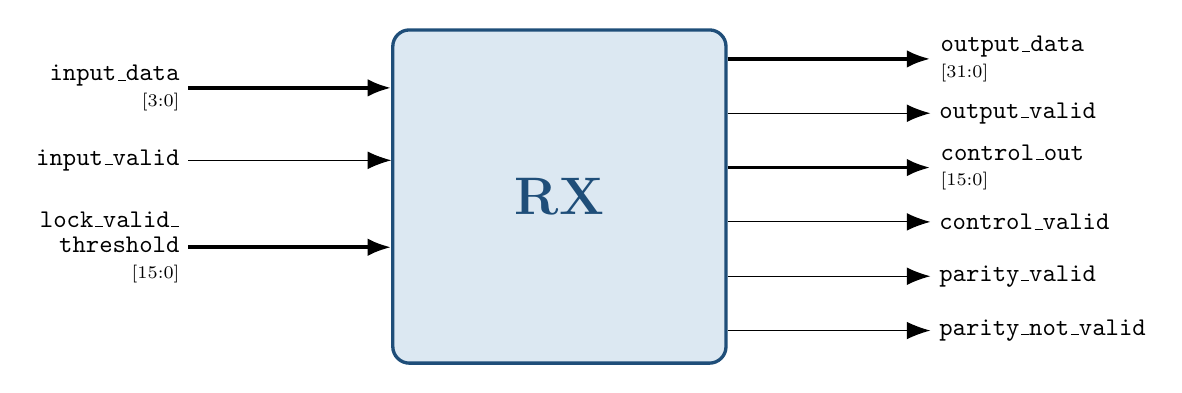
\begin{tikzpicture}[>=Latex, scale=0.92, every node/.style={scale=0.92}]
  \RXDiagram
\end{tikzpicture}
\end{center}

\vspace{2.4cm}

\begin{center}
\begin{tabular}{L{3.2cm}L{7cm}}
\toprule
\textbf{Document} & RX RTL Specification \\
\textbf{Block} & DMA Receiver (RX) \\
\textbf{Scope} & RTL functional behavior only (no verification content) \\
\textbf{Date} & \today \\
\bottomrule
\end{tabular}
\end{center}

\restoregeometry
\end{titlepage}

\tableofcontents
\newpage

% ===========================================================================
\section{Overview}
% ===========================================================================
The \textbf{RX} block receives a continuous stream of packets on a narrow
input bus and reconstructs the \emph{Data} and \emph{Control} payload that
each packet carries. Because the packet boundary is not aligned with the
input bus a priori, the module must first \emph{discover} where packets
begin (the \emph{phase}), lock onto that phase once it is confident, and
only then start emitting decoded data.

Once locked, the module tolerates a single-bit error in either the
\texttt{LENGTH} field or the \texttt{CONTROL} field of a packet (each
protected by its own 16-bit CRC) by correcting it in place, and it reports
the parity health of every packet it outputs.

\begin{noteBox}[Key responsibilities]
\begin{itemize}[leftmargin=1.4em, itemsep=2pt]
  \item Discover and lock the packet phase on an unaligned nibble stream.
  \item Extract \texttt{LENGTH}, \texttt{CONTROL} and \texttt{DATA} from every packet.
  \item Detect and correct single-bit errors in \texttt{LENGTH} and \texttt{CONTROL}.
  \item Validate end-to-end packet parity and flag the result.
  \item Suppress \texttt{CONTROL} output when its value is zero.
\end{itemize}
\end{noteBox}

% ===========================================================================
\section{Interface}
% ===========================================================================

\subsection{Block Diagram}
Signals drawn with a thick arrow are multi-bit buses; signals drawn with a
thin arrow are single-bit strobes / indications.

\begin{center}
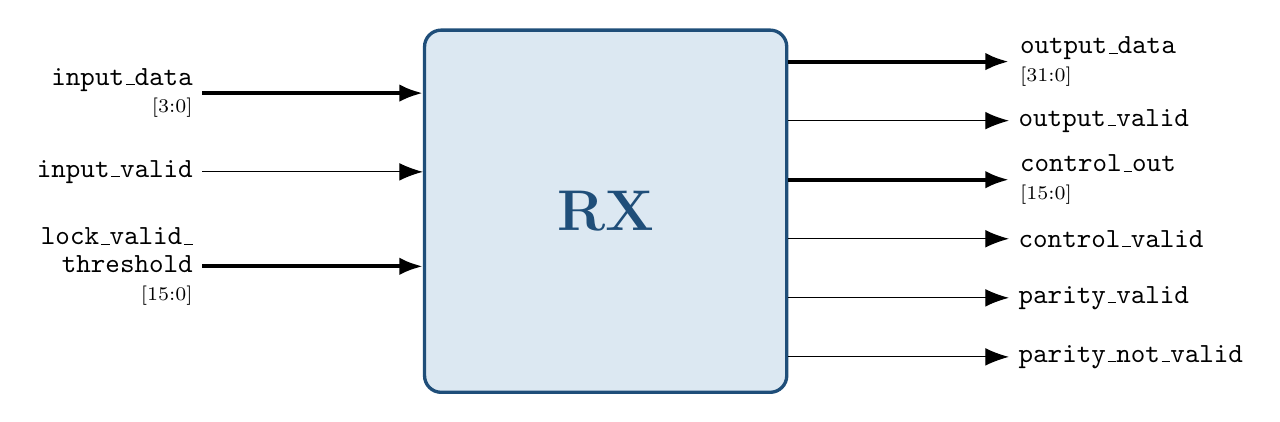
\begin{tikzpicture}[>=Latex]
  \RXDiagram
\end{tikzpicture}
\end{center}

\subsection{Parameters}
\begin{center}
\footnotesize
\begin{tabular}{L{4.4cm}C{1.6cm}L{7.4cm}}
\toprule
\textbf{Parameter} & \textbf{Default} & \textbf{Description / Legal range} \\
\midrule
\path{INPUT_DATA_WIDTH} & 4 & Width of the incoming data bus, in bits. \\
\path{LOCK_THRESHOLD_DATA_WIDTH} & 16 & Width of the lock-threshold bus, in bits. \\
\path{OUTPUT_DATA_WIDTH} & 32 & Width of the outgoing data bus, in bits. \\
\path{CONTROL_DATA_WIDTH} & 16 & Width of the outgoing control bus, in bits. \\
\bottomrule
\end{tabular}
\end{center}

\subsection{Ports}
\begin{center}
\footnotesize
\begin{tabular}{L{2.9cm}C{1.0cm}C{2.6cm}L{6.9cm}}
\toprule
\textbf{Signal} & \textbf{I/O} & \textbf{Width} & \textbf{Description} \\
\midrule
\path{input_data} & in & \path{INPUT_DATA_WIDTH} & Incoming packet stream. \\
\path{input_valid} & in & 1 & Qualifies \path{input_data} as valid on this cycle. \\
\path{lock_valid_threshold} & in & \path{LOCK_THRESHOLD_DATA_WIDTH} & Number of consecutive valid packets required, at the same phase, before the module locks. \\
\path{output_data} & out & \path{OUTPUT_DATA_WIDTH} & Decoded \texttt{DATA} payload of the current packet. \\
\path{output_valid} & out & 1 & Qualifies \path{output_data} as valid on this cycle. \\
\path{control_out} & out & \path{CONTROL_DATA_WIDTH} & Decoded \texttt{CONTROL} field of the current packet. \\
\path{control_valid} & out & 1 & Qualifies \path{control_out} as valid (never asserted when \path{control_out} is all-zero). \\
\path{parity_valid} & out & 1 & The packet's parity checked correct. \\
\path{parity_not_valid} & out & 1 & The packet's parity checked incorrect. \\
\bottomrule
\end{tabular}
\end{center}

% ===========================================================================
\section{Packet Format}
% ===========================================================================
Every packet on \texttt{input\_data} has the following structure:

\begin{center}
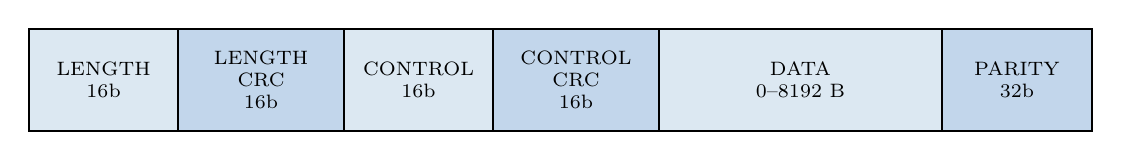
\begin{tikzpicture}[font=\scriptsize]
  \def\h{1.3}
  \newcommand{\field}[3]{
    \draw[thick, fill=#3] (\cx,0) rectangle ++(#1,\h);
    \node[align=center] at (\cx+#1/2,\h/2) {#2};
    \pgfmathsetmacro{\cx}{\cx+#1}
  }
  \pgfmathsetmacro{\cx}{0}
  \field{1.9}{LENGTH\\16b}{accentlight}
  \field{2.1}{LENGTH\\CRC\\16b}{accentmid!40}
  \field{1.9}{CONTROL\\16b}{accentlight}
  \field{2.1}{CONTROL\\CRC\\16b}{accentmid!40}
  \field{3.6}{DATA\\0--8192 B}{accentlight}
  \field{1.9}{PARITY\\32b}{accentmid!40}
\end{tikzpicture}
\end{center}

\begin{itemize}[leftmargin=1.4em, itemsep=3pt]
  \item \texttt{LENGTH} is expressed in \textbf{bytes} and equals the size of
        \texttt{DATA} plus the size of \texttt{CONTROL} and
        \texttt{CONTROL\_CRC}: \texttt{LENGTH = len(DATA) + 4}.
  \item \texttt{DATA} length must always be a multiple of 32 bits ---
        since \texttt{LENGTH} is expressed in bytes (4 bytes = 32 bits),
        this means \texttt{LENGTH} itself must always be a multiple of 4.
  \item \texttt{PARITY} is the running XOR of every 32-bit word of the
        \texttt{DATA} field.
  \item If the (corrected) value of \texttt{CONTROL} is zero, it is not
        driven out on \texttt{control\_out} / \texttt{control\_valid}.
\end{itemize}

% ===========================================================================
\section{Functional Behavior}
% ===========================================================================

\subsection{Phase Acquisition and Lock}
The first bit of a packet is not necessarily the first bit sampled on
\texttt{input\_data} --- a packet may start at any nibble offset within the
bus word. On reset, the module does not know this offset (the
\emph{phase}) and must search for it.

\textbf{Search.} For every candidate phase (one of \texttt{INPUT\_DATA\_WIDTH}
possible nibble offsets), the module continuously computes the CRC of a
32-bit sliding window and compares it against the \texttt{LENGTH\_CRC} that
would accompany it. A phase is a candidate match the moment its computed
\texttt{LENGTH\_CRC} agrees with the field carried in the stream.

\textbf{Confirmation.} The module keeps re-checking the candidate phase on
every subsequent packet. Once the \emph{same} phase has produced a valid
(\texttt{LENGTH}, \texttt{LENGTH\_CRC}) pair for \texttt{lock\_valid\_threshold}
consecutive packets, the phase is considered found and the module locks
onto it permanently (until reset). Any packet received while the phase is
still being searched for is dropped. A single invalid packet while
confirming resets the consecutive count and returns the search to
\texttt{NOT\_LOCKED}.

\begin{center}
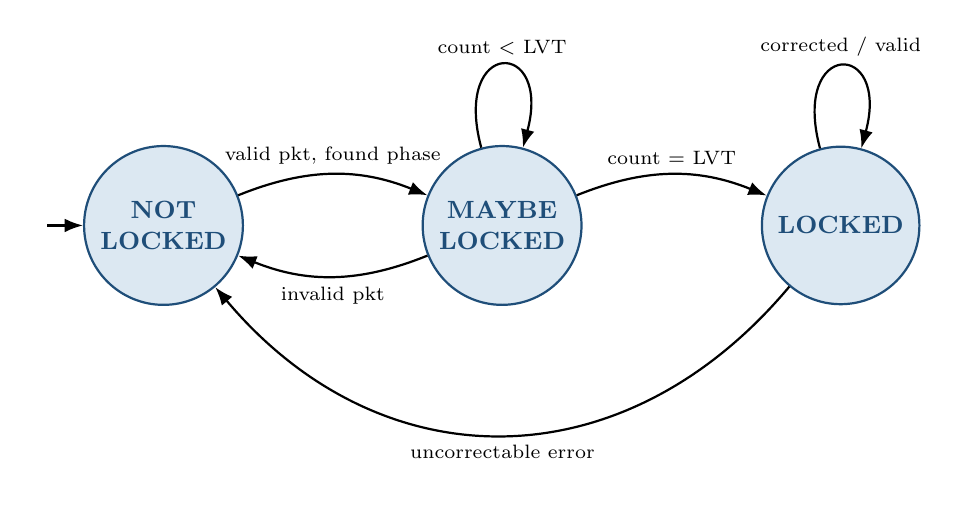
\begin{tikzpicture}[
  >=Latex, node distance=4.3cm, on grid, auto,
  every state/.style={draw=accent, thick, fill=accentlight, text=accent,
                       minimum size=2.0cm, font=\small\bfseries,
                       align=center},
  every edge/.style={draw, thick},
  every edge/.append style={font=\scriptsize}
]
  \node[state, initial, initial text=] (nl)              {NOT\\LOCKED};
  \node[state]                          (ml) [right=of nl] {MAYBE\\LOCKED};
  \node[state]                          (lk) [right=of ml] {LOCKED};

  \path[->]
    (nl) edge[bend left=22]            node[above]{valid pkt, found phase} (ml)
    (ml) edge[bend left=22]            node[below]{invalid pkt} (nl)
    (ml) edge[loop above, looseness=7] node[above]{count $<$ LVT} (ml)
    (ml) edge[bend left=22]            node[above]{count = LVT} (lk)
    (lk) edge[loop above, looseness=7] node[above]{corrected / valid} (lk)
    (lk) edge[bend left=50, looseness=1.15] node[below]{uncorrectable error} (nl);
\end{tikzpicture}
\end{center}

\subsection{Single-Bit Error Correction}
Once \texttt{LOCKED}, the module accepts and corrects packets carrying
\emph{at most one} bit error in \path{LENGTH/LENGTH_CRC}
\textbf{or} in \path{CONTROL/CONTROL_CRC}: the syndrome of the
32-bit window is matched against the field's single-bit-error signature,
the affected bit is flipped, and the corrected value is used downstream.
Correction is only attempted after lock; before lock, any CRC mismatch
simply fails the phase-search check described above.

\subsection{Parity Validation}
For every packet, the module accumulates the XOR of all 32-bit \texttt{DATA}
words and compares it against the trailing 32-bit \texttt{PARITY} field,
raising exactly one of \texttt{parity\_valid} / \texttt{parity\_not\_valid}.
Parity is a pure indication --- it does not gate whether \texttt{output\_data}
is driven.

\subsection{Output Control Gating}
\texttt{control\_out} / \texttt{control\_valid} are only asserted when the
(possibly corrected) \texttt{CONTROL} value is non-zero; an all-zero
\texttt{CONTROL} field is treated as ``no control for this packet'' and is
never presented on the output bus.

% ===========================================================================
\section{CRC Specification}
% ===========================================================================

\subsection{Data Window Format}
Both CRC checks operate on a 32-bit window:
\[
  \texttt{window[31:16]} = \text{data\_field}, \qquad
  \texttt{window[15:0]} = \text{crc\_field}.
\]
The CRC is computed over the 16-bit \texttt{data\_field}, MSB-first
(from bit~15 down to bit~0), and compared against \texttt{crc\_field}.
Both fields share the generic engine
\texttt{calculate\_crc16\_generic(data, polynomial, init\_val)}.

\subsection{Length CRC --- CRC-16-CCITT}
\begin{center}
\begin{tabular}{ll}
\toprule
Polynomial & \texttt{0x1021} \\
Initial value & \texttt{0xFFFF} \\
\bottomrule
\end{tabular}
\end{center}

\subsection{Control CRC --- CRC-16-IBM/ANSI}
\begin{center}
\begin{tabular}{ll}
\toprule
Polynomial & \texttt{0x8005} \\
Initial value & \texttt{0x0000} \\
\bottomrule
\end{tabular}
\end{center}

% ===========================================================================
\section{Throughput Requirement}
% ===========================================================================
The module shall sustain \textbf{1\,Gbit/s} of incoming payload data on a
4-bit input bus clocked at \textbf{1\,GHz}.

% ===========================================================================
\section{System-Level Assumptions}
% ===========================================================================
The following are preconditions the module relies on for correct operation
--- they are not behaviors the RTL derives on its own, but constraints the
surrounding system and traffic generator must uphold.

\begin{sysBox}[SYS-01 --- Payload alignment]
Data payload length is always a multiple of 4 bytes.\\
\textit{Rationale: parity is a 32-bit word and the output data bus is 32 bits wide.}
\end{sysBox}

\begin{sysBox}[SYS-02 --- Lock retention]
Once the module reaches \texttt{LOCKED}, it is assumed to never need to drop
out of lock.\\
\textit{Rationale: after lock, at most one bit error is assumed in
\texttt{LENGTH} + \texttt{LENGTH\_CRC} per packet; two or more simultaneous
errors after lock fall outside the specified operating envelope (the RTL
will fall back to \texttt{NOT\_LOCKED} and re-search in that case, but this
is not a scenario the module is required to handle gracefully).}
\end{sysBox}

\begin{sysBox}[SYS-03 --- Static lock threshold]
\texttt{lock\_valid\_threshold} (LVT) is configured once, at the start of
operation, and never changes for the lifetime of the lock.\\
\textit{Legal range: $2 \le \text{LVT} \le 12$. The port itself is 16 bits wide.}
\end{sysBox}

\begin{sysBox}[SYS-04 --- Maximum payload size]
Data payload length is at most 8\,KB.\\
\textit{The maximum payload is 8192 bytes; the \texttt{LENGTH} field is 16
bits wide (payload alone does not use its full numeric range).}
\end{sysBox}

\begin{ruleBox}[Note]
SYS-02 is an operating assumption, not a hard guarantee: the lock FSM in
\texttt{dma\_rx\_fsm.sv} does return to \texttt{NOT\_LOCKED} on an
uncorrectable \texttt{LENGTH} CRC failure while locked. The assumption
states that, under normal (single-bit-error) conditions, this path is not
expected to trigger.
\end{ruleBox}

\end{document}
